\documentclass{standalone}
\usepackage{tikz}
\usepackage{ctex,siunitx}
\setCJKmainfont{Noto Serif CJK SC}
\usepackage{tkz-euclide}
\usepackage{amsmath}
\usepackage{wasysym}
\usetikzlibrary{patterns, calc}
\usetikzlibrary {decorations.pathmorphing, decorations.pathreplacing, decorations.shapes,}
\begin{document}
\small
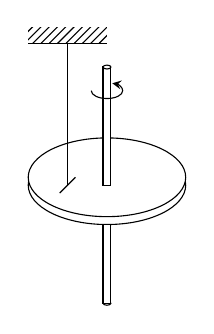
\begin{tikzpicture}[>=stealth,scale=1]
  \fill[pattern=north east lines](-1,1.8) rectangle (0,2);
  \draw(-1,1.8)--(0,1.8);
  \draw(0,0)ellipse[x radius=1, y radius=.5];
  \draw[fill=white](0,0.1)ellipse[x radius=1, y radius=.5];
  \draw(-.5,1.8)--(-.5,0);
  \draw(-.6,-.1)--(-.4,0.1);
  \draw[fill=white](-.05,0) rectangle (.05,1.5);
  \draw[fill=white](0,-1.5)ellipse[x radius=.05, y radius=.025];
  \draw[fill=white](-.05,-.5) rectangle (.05,-1.5);
  \draw[fill=white](0,1.5)ellipse[x radius=.05, y radius=.025];
  \draw[->](-.2,1.2) arc [start angle =-180, end angle =70, x radius=.2, y radius=.1];
\end{tikzpicture}
\end{document}